\documentclass[tikz]{standalone}
\usepackage{amssymb,dsfont}
\usepackage{color}
\usetikzlibrary{arrows}
% Sets
\newcommand{\CC}{\mathbb{C}}        % Complex numbers
\newcommand{\NN}{\mathbb{N}}        % Natural numbers
\newcommand{\RR}{\mathbb{R}}        % Real numbers
\newcommand{\ZZ}{\mathbb{Z}}        % Relative integers
% Groups
\newcommand{\SO}{\mathrm{SO}}       % Special orthogonal group
\newcommand{\OO}{\mathrm{O}}        % Orthogonal group
\newcommand{\SU}{\mathrm{SU}}       % Special unitary group
\newcommand{\1}{\mathds{1}}		    % trivial group
\newcommand{\DD}{\mathbb{D}}        % Dihedral group
\newcommand{\octa}{\mathbb{O}}      % Cubic (octahedral) group
\newcommand{\ico}{\mathbb{I}}       % Icosahedral group
\newcommand{\tetra}{\mathbb{T}}     % tetrahedral group
\begin{document}
	
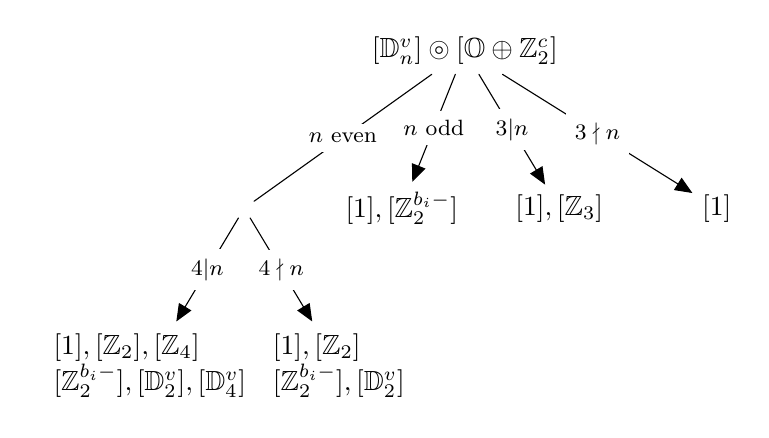
\begin{tikzpicture}[scale=0.8,line cap=round,line join=round,>=triangle 45,x=1.0cm,y=1.0cm]
  \node (root) at (0,0) {$[\DD_n^v]\circledcirc [\octa\oplus \ZZ_2^c]$};

  \node (Bas1) at (-3.5,-2.5) {};
  \node (Bas2) at (-1,-2.5)   {$[\1],[\ZZ_2^{b_i-}]$};
  \node (Bas3) at (1.5,-2.5) {$[\1],[\ZZ_3]$};
  \node (Bas4) at (4,-2.5) {$[\1]$};
  \draw (root) -- (Bas1) node [midway,fill=white] {{\footnotesize $n$ even }};
  \draw [->](root) -- (Bas2) node [midway,fill=white] {{\footnotesize  $n$ odd}};
  \draw [->](root) -- (Bas3) node [midway,fill=white] {{\footnotesize  $3|n$}};
  \draw [->](root) -- (Bas4) node [midway,fill=white] {{\footnotesize  $3 \nmid n$}};
  \node (Bas11) at (-3.5-1.5,-5) {\begin{tabular}{l} $[\1],[\ZZ_2],[\ZZ_4]$ \\ $[\ZZ_2^{b_i-}],[\DD_2^v],[\DD_4^v]$\end{tabular}};
  \node (Bas12) at (-3.5+1.5,-5) {\begin{tabular}{l} $[\1],[\ZZ_2]$ \\ $[\ZZ_2^{b_i-}],[\DD_2^v]$\end{tabular}};
  \draw[->] (Bas1) -- (Bas11) node [midway,fill=white] {{\footnotesize $4|n$}};
  \draw[->] (Bas1) -- (Bas12) node [midway,fill=white] {{\footnotesize $4 \nmid n$}};
\end{tikzpicture}
% Further ’tikzpicture’ environments are possible which will create further pages.
\end{document} 